\documentclass{standalone}
\usepackage{tikz}
\usepackage{fontspec}

\newcommand{\ceva}[1]{ {\fontspec{[ceva-c2.ttf]}#1}}
\newcommand{\cevain}[1]{ {\fontspec{[ceva-c2.ttf]}#1} | \emph{#1}}

\begin{document}
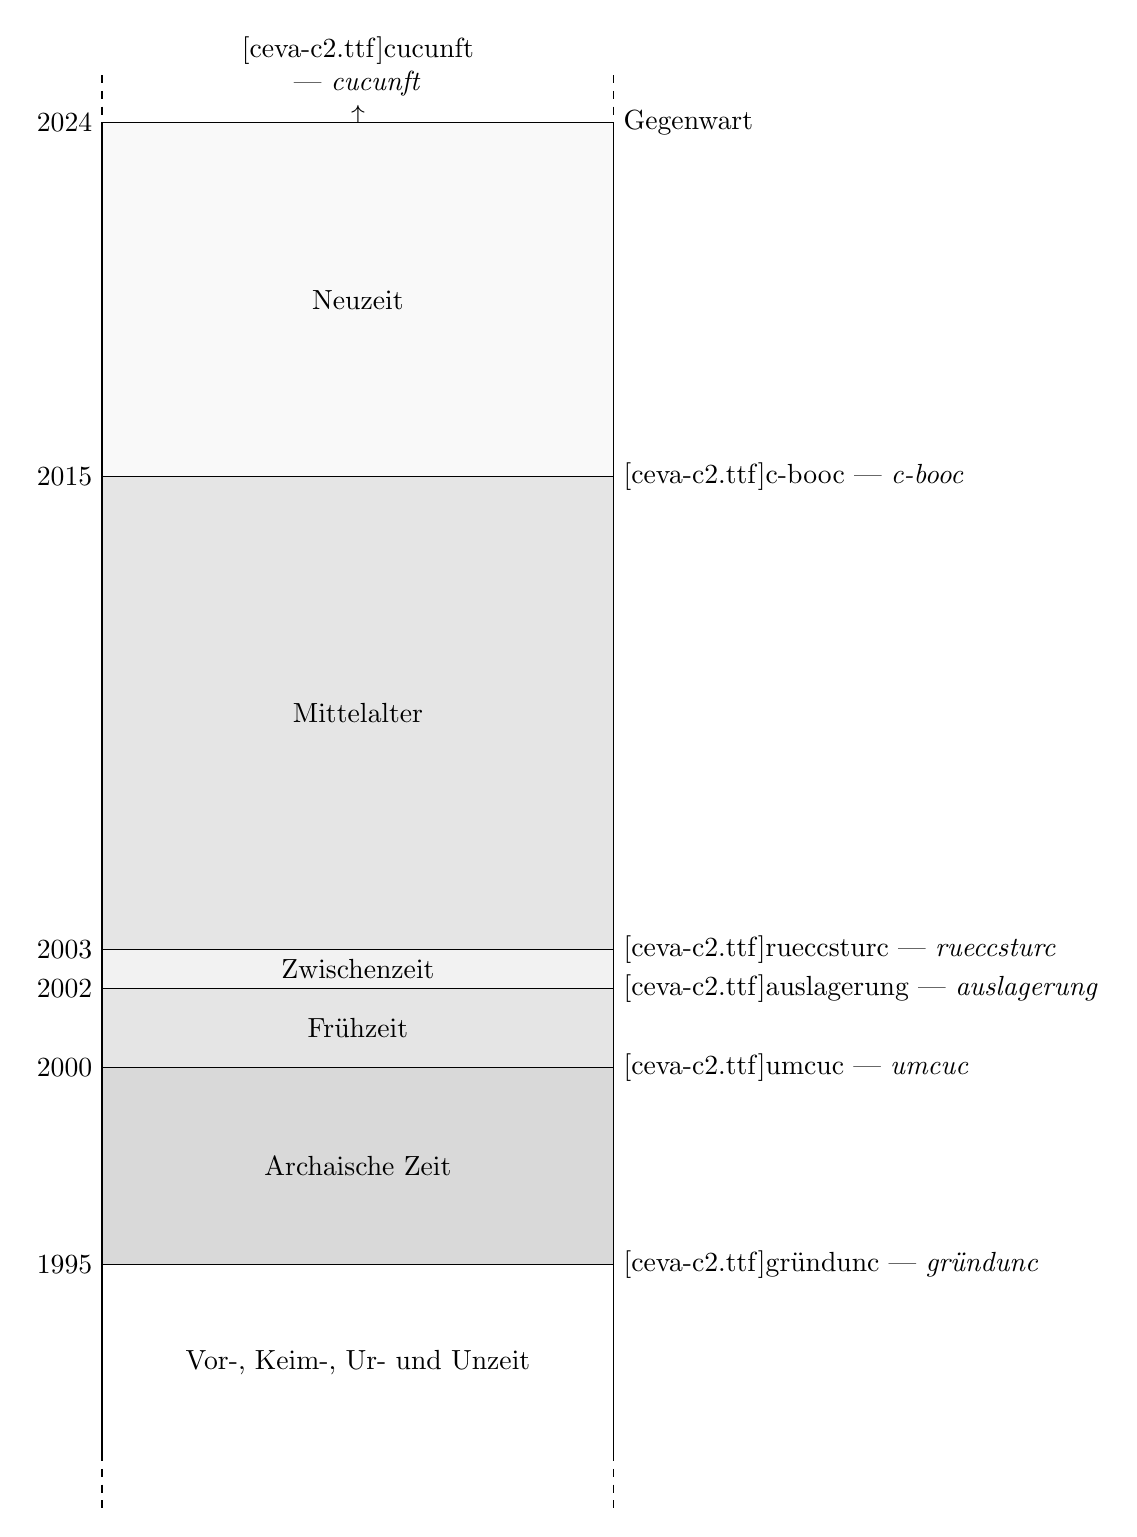
\begin{tikzpicture}[yscale=0.5,xscale=1.3]
    % \draw (0) rectangle (0,,1);
    \foreach \i in {124.4,124.8,125.2} 
        {
        \draw (0,\i) -- (0,\i-0.2);
        \draw (5,\i) -- (5,\i-0.2);
        }

    \node at (2.5,125) {\parbox{20ex}{\centering\cevain{cucunft}\\ $\uparrow$ }};
    
    \node [right] at (5,124) {Gegenwart};
    
    \draw[fill=gray!5] (0,124) node [left] {2024} rectangle node {Neuzeit} (5,115) node [right] {\cevain{c-booc}};
    % \draw (0,115) -- (0,124); draw (5,114) -- (5,124); \draw (0,115
    
    \draw[fill=gray!20] (0,115) node [left] {2015} rectangle node {Mittelalter} (5,103) node [right] {\cevain{rueccsturc}};
    
    \draw[fill=gray!10] (0,103)  node [left] {2003} rectangle node {Zwischenzeit} (5,102) node [right] {\cevain{auslagerung}};
    
    \draw[fill=gray!20] (0,102)  node [left] {2002} rectangle node {Frühzeit} (5,100) node [right] {\cevain{umcuc}};
    
    \draw[fill=gray!30] (0,100)  node [left] {2000} rectangle node {Archaische Zeit} (5,95) node [right] {\cevain{gründunc}};
    % \node at (0,95) [left] {1995};
    
    \draw[draw=none] (0,95)  node [left] {1995} rectangle node {Vor-, Keim-, Ur- und Unzeit} (5,90) ;
    \draw (0,95) -- (0,90); \draw (5,95) -- (5,90);
    
    \foreach \i in {89.8,89.4,89} 
        {
        \draw (0,\i) -- (0,\i-0.2);
        \draw (5,\i) -- (5,\i-0.2);
        }
    
    
    % \draw[<->] (0,95) rectangle (0,65);
\end{tikzpicture}

\end{document}
